\chapter{Motivating Scenario}
\label{chap:motivatingScenario}
In order to help in understanding the concepts of organizational modeling, a motivating scenario has been taken and explained through the modeling notations mentioned in the Section \ref{sec:resourcecentricorganizationalmodeling} of Chapter \ref{chap:fundamentals}. This scenario also helps to validate the developed web-based modeling tool in the Section \ref{sec:validation} of Chapter \ref{chap:casestudy}. The motivating scenario has been chosen based on the collected real life scenarios provided in another thesis work \cite{Sierr2015}. The motivating scenario is taken from the context of manufacturing sector. 

In this chapter, the first section provides a brief introduction about the motivating scenario. The last section provides an explanation about the organizational modeling elements discussed in the motivating scenario. 
%%%%%%%%%%%%%%%%%%%%%%%%%%%%%%%%%%%%%%%%%%%%%%%%%%%%%%%%%%%%%%%%%%%%%%%%%
\section{Intention-oriented Organizational Modeling Example}
\label{sec:scenario}
%%%%%%%%%%%%%%%%%%%%%%%%%%%%%%%%%%%%%%%%%%%%%%%%%%%%%%%%%%%%%%%%%%%%%%%%%
The concept of intention oriented organizational modeling can be explained with the following scenario taken from a manufacturing organization. Consider a budding manufacturing company which designs, develops, manufactures and sells personal computers and laptops. The CEO's main intention of the quarter is \textit{to increase the revenue and number of unit sales}. Intentions connect initial context definitions with final context definitions \cite{Sungur2014a}. There are also low level intentions other than the main intention which helps in achieving main intention as a collection of several intentions in a measurable form. 
 
\begin{figure}
  	\centering
  	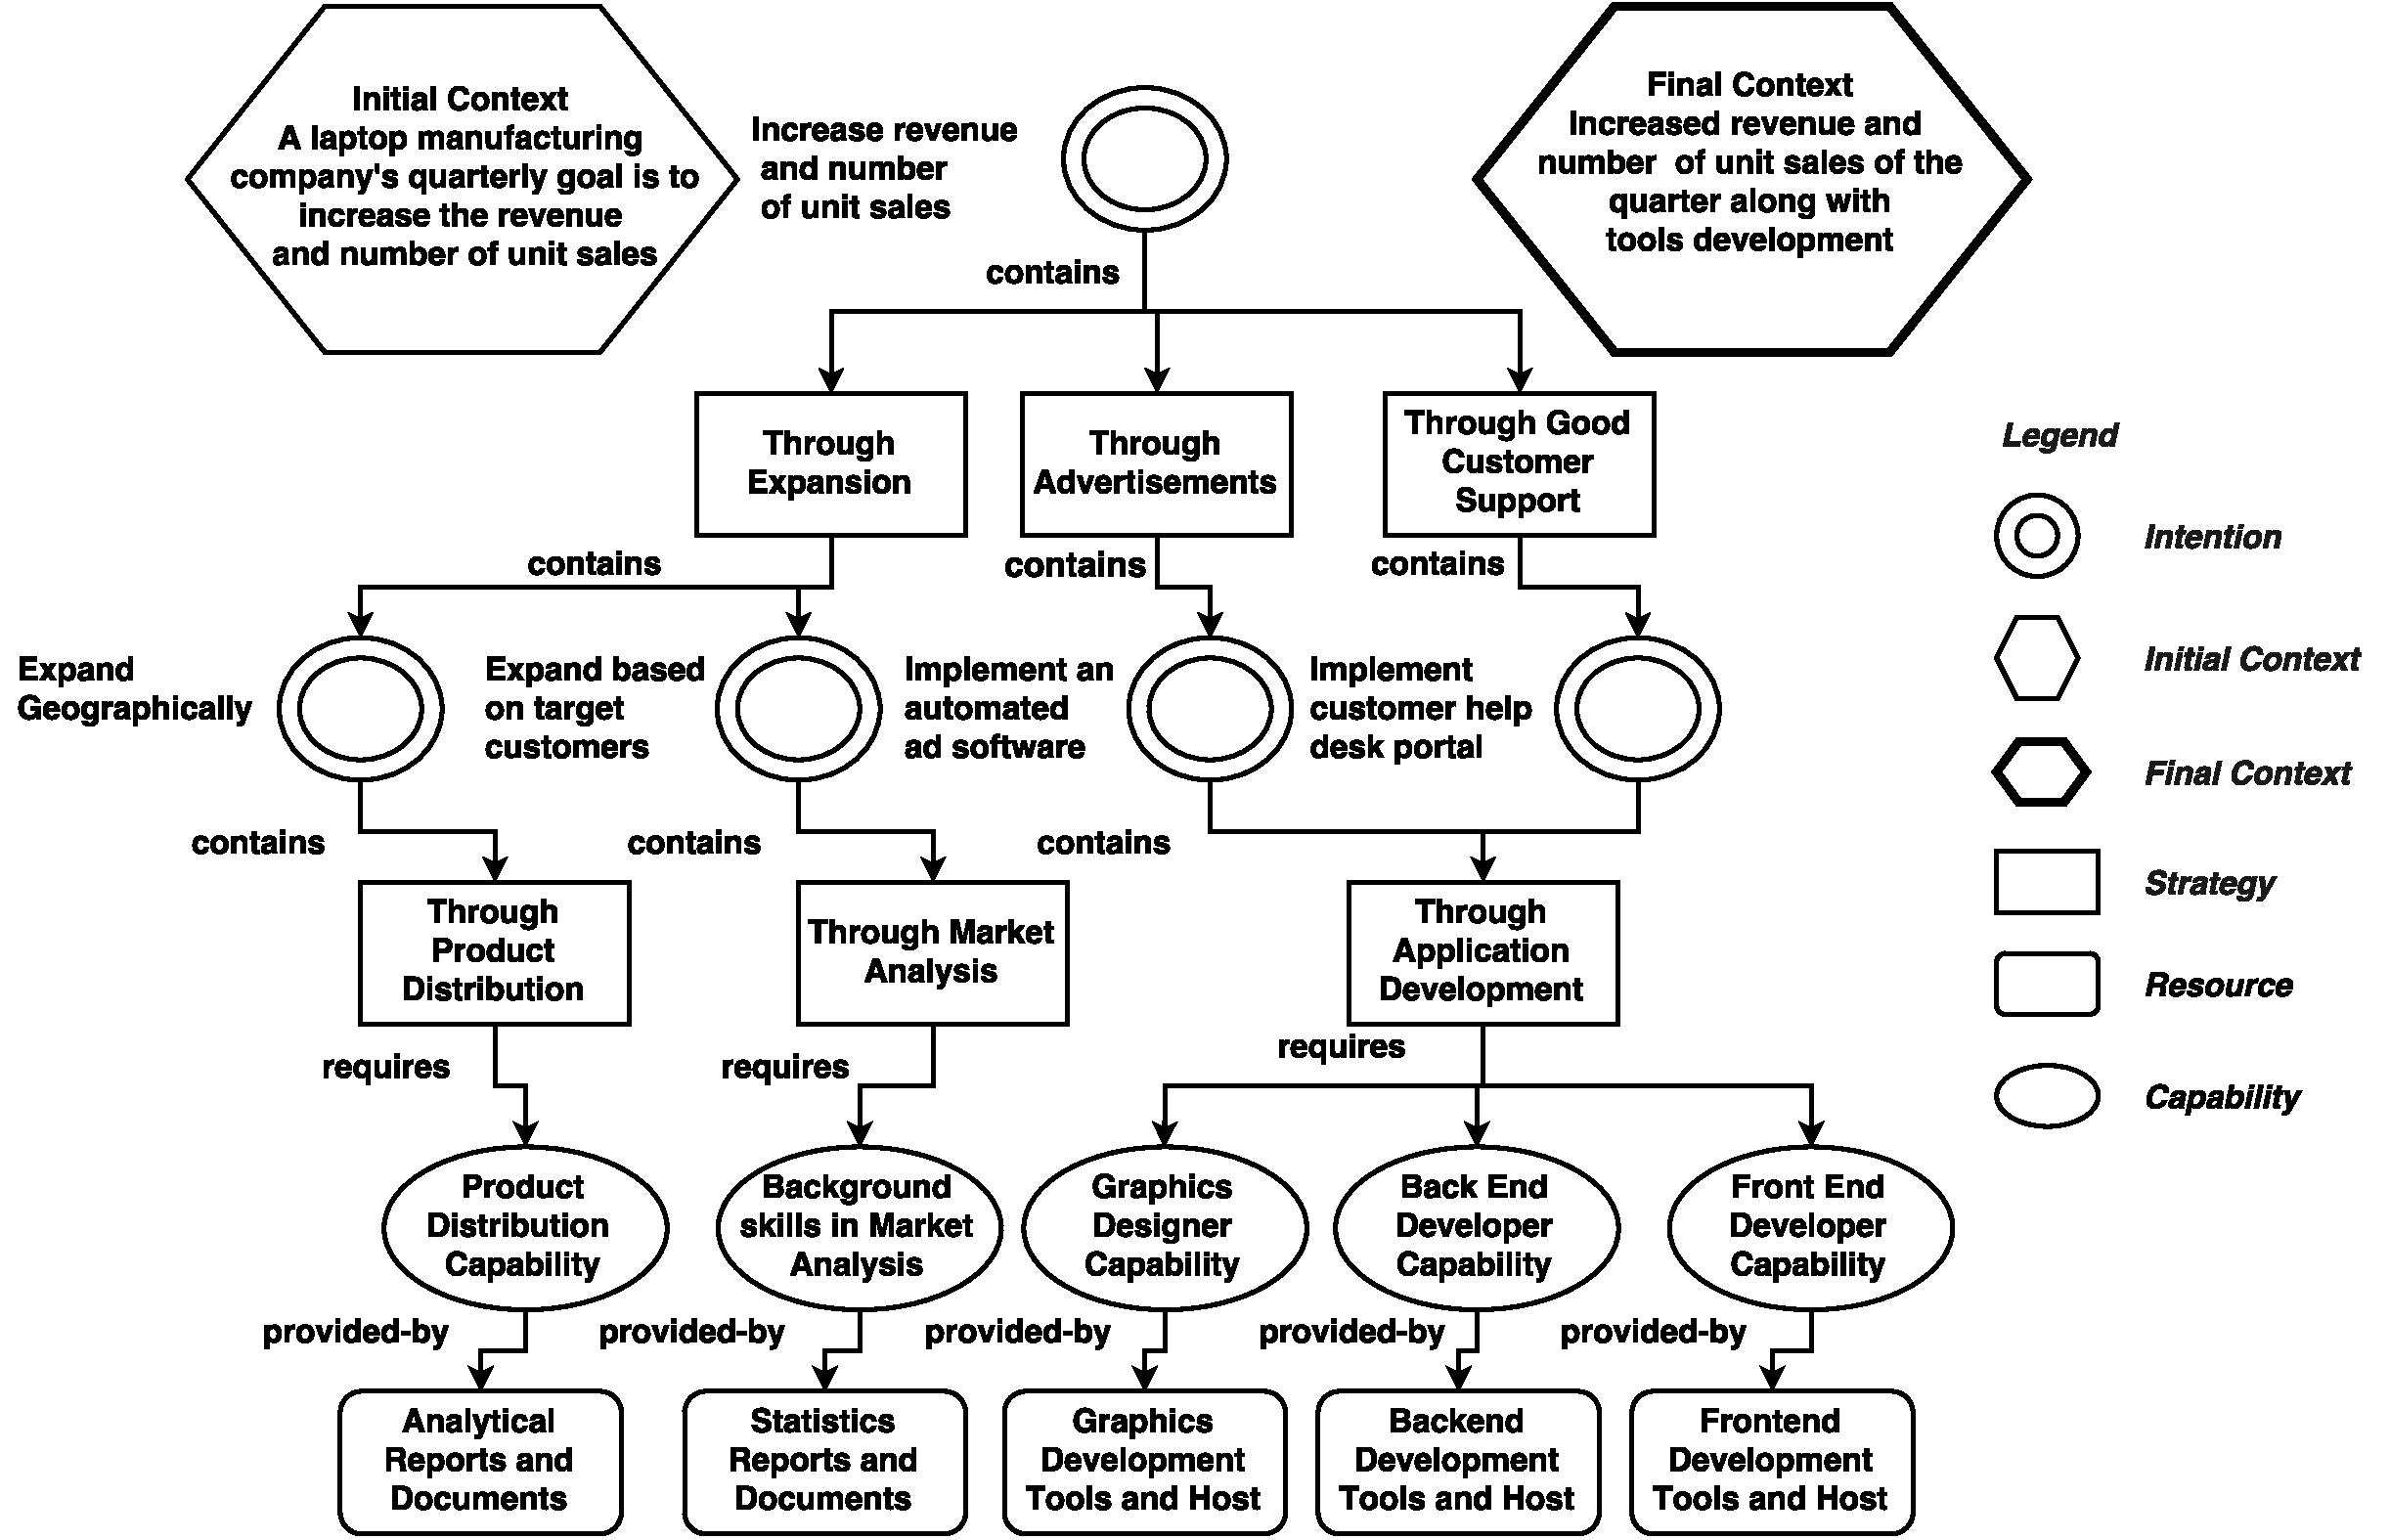
\includegraphics[width=\textwidth,angle=0]{MotivatingScenario.pdf}
  	\caption{Intention-oriented Organizational Modeling - Example Scenario}
  	\label{fig:motivatingscenario}
\end{figure}
  
The Figure \ref{fig:motivatingscenario} provides the details of organizational intentions, strategies, capabilities and resources. There can be multiple strategies followed to achieve a main intention. The main intention in the motivating scenario can be achieved by following all of the below mentioned strategies. These strategies require resources with matching capabilities.
 
 \begin{enumerate}
 	\item Through increasing the revenue by expanding the market sales. 
 	\item Through increasing advertisements, which helps the customer to know about the product.
 	\item Through improving the existing customer help desk portal, as it helps to maintain good customer relationship.
 \end{enumerate}
 
%%%%%%%%%%%%%%%%%%%%%%%%%%%%%%%%%%%%%%%%%%%%%%%%%%%%%%%%%%%%%%%%%%%%%%%%%
\section{Intention-oriented Organizational Modeling Elements}
\label{sec:entities}
%%%%%%%%%%%%%%%%%%%%%%%%%%%%%%%%%%%%%%%%%%%%%%%%%%%%%%%%%%%%%%%%%%%%%%%%%
It is important to explain each of the organizational modeling element using an example, as it helps in understanding the requirements of intention-oriented organizational modeling discussed in the Section \ref{sec:requirementssupoorting}. Before we proceed with detailed description of each modeling element, we provide an example scenario to know the dynamic nature of the organizational modeling. For example, in our above mentioned motivating scenario in the Section \ref{sec:scenario} one of the intention is to \textit{expand sales geographically}. To achieve this intention successfully, few ground works like collection of laptop usage statistics such as average buying capacity of the consumers, average computer knowledge of the people in new geographic location has to be done. Thus, the main intention, i.e., \textit{increase revenue and number of unit sales}, requires collaboration of people with different skills and expertise. For example, resources with capability to do market analysis are required. If in case none of the organizational resources provide required capability, then the organization can get it served from external resources or further modularize the intention so that it can be provided by internal resources itself. This makes to emerge new intentions dynamically. The team working towards achievement of main intention should also be ready to accommodate new resources with new capabilities and skills. For example, there is a software development team, which work towards achievement of the intention \textit{improve customer help desk portal}, i.e., this team develops software that automatically attends and records user queries. Suppose, if there arise a new requirement of \textit{supporting help desk through mobile applications} then the system should accommodate new resource with \textit{mobile application developer} capability. 

%%%%%%%%%%%%%%%%%%%%%%%%%%%%%%%%%%%%%%%%%%%%%%%%%%%%%%%%%%%%%%%%%%%%%%%%%
\subsection{Contexts} 
\label{sec:contexts}
%%%%%%%%%%%%%%%%%%%%%%%%%%%%%%%%%%%%%%%%%%%%%%%%%%%%%%%%%%%%%%%%%%%%%%%%%
The execution of the manufacturing processes such as the one provided in Figure \ref{fig:motivatingscenario} are not similar to execution of typical business processes. This is because, the execution of manufacturing processes mostly depends on the information collected from the real world, i.e., the execution context \cite{Sungur2016}. A context definition provides mechanism to act adaptively based on the current situation. This is achieved in the production environment by describing each process with a specific context definition \cite{Sungur2016}. For example, in our motivating scenario the initial context provides details about status before achievement of the main intention, i.e., it specifies the situation of the organization which triggers the execution of main-intention. The actual problem context is, the revenue of the previous quarter was lesser than the estimated revenue. Hence, the initial context for next quarter is set as \textit{quarterly goal of increasing the revenue and number of unit sales}. The initial context helps to decide the main intention and its related low level associates. On successful achievement of main-intention, the intention reaches desired state which is called as final context. Along with successful reaching of the final context, this also provides tools such as web-based help desk portals, automated ad software etc., that are developed as part of this intention achievement. When the final context definition has been reached the process completion starts. This process final state can be stored and same set of resources can be re-used in future executions with similar contexts and intentions \cite{Sungur2015}.
 
%%%%%%%%%%%%%%%%%%%%%%%%%%%%%%%%%%%%%%%%%%%%%%%%%%%%%%%%%%%%%%%%%%%%%%%%%
\subsection{Intentions} 
\label{sec:intentions}
%%%%%%%%%%%%%%%%%%%%%%%%%%%%%%%%%%%%%%%%%%%%%%%%%%%%%%%%%%%%%%%%%%%%%%%%%
The intentions are defined hierarchically in the motivating scenario. The intentions are located at top level of the hierarchy, which are refined until concrete lower level of the hierarchy is reached. In the motivating scenario, intentions are not associated with capabilities directly, instead intentions are associated with strategies which are then associated with capabilities. For example, in our motivating scenario the main intention is to increase revenue and number of unit sales which also has other low level intentions such as \textit{improving the customer help desk portal} and strategies such as (1) through expanding sales and (2) through advertisements. The relation between strategies and intentions are denoted by the term \textit{contains} in Figure \ref{fig:motivatingscenario}. This because through strategies, intentions can be achieved. There can be situation where an intention can be related to another intention. There can be custom relationships between intentions such as contains, contradicts, etc. For example, consider in our motivating scenario the intention \textit{implement an automated ad software} can also contain an intention \textit{implement a mobile application}.  

%%%%%%%%%%%%%%%%%%%%%%%%%%%%%%%%%%%%%%%%%%%%%%%%%%%%%%%%%%%%%%%%%%%%%%%%%
\subsection{Strategies} 
\label{sec:strategies}
%%%%%%%%%%%%%%%%%%%%%%%%%%%%%%%%%%%%%%%%%%%%%%%%%%%%%%%%%%%%%%%%%%%%%%%%%
As mentioned earlier, a strategy is an approach, a manner or a means to achieve an intention \cite{Bider2005}. Strategies are associated with both intentions and capabilities. Each strategy needs certain capabilities to successfully accomplish an intention. We need to associate strategy with a capability that has matching resource. The resources are the potential holder of the capability, i.e., to satisfy a capability we need resources. The capability and its associated resources are also shown in the Figure \ref{fig:motivatingscenario}. In our motivating scenario, the main intention can be achieved through two strategies \textit{through expansion} and \textit{through advertisements}. These two strategies further contain the intentions such as \textit{expand geographically}, \textit{expand based on target customers} and \textit{implement an automated ad software}. Since, strategies contain intentions they are related through the term \textit{contains} in the Figure \ref{fig:motivatingscenario}. As mentioned earlier, the informal process models are realized through strategies. This is achieved through strategy containing capabilities and resources. For example, consider a small part in our motivating scenario of achieving an intention \textit{expand geographically} through strategy \textit{product sales distribution}. This strategy is chosen because the products will reach customer only if it is effectively distributed. To achieve this intention, through a specified strategy we need resources with the product sales distribution capability, i.e., resources that has an ability to effectively distribute the products. For example, sales agents, wholesalers or other kinds of sales distributors. 

%%%%%%%%%%%%%%%%%%%%%%%%%%%%%%%%%%%%%%%%%%%%%%%%%%%%%%%%%%%%%%%%%%%%%%%%%
\subsection{Capabilities}
\label{sec:capabilities}
%%%%%%%%%%%%%%%%%%%%%%%%%%%%%%%%%%%%%%%%%%%%%%%%%%%%%%%%%%%%%%%%%%%%%%%%%
The organizational resources posses certain capabilities to work towards the achievement of an intention. Each organizational capability must be provided by a resource in the organization. In our context, capabilities that are associated with resources are called as \textit{functional capabilities}. The type of capability that contains functional capabilities are called as \textit{cross-functional capabilities}. Strategies are associated with cross-functional capabilities, which contains functional capabilities out of which resources are created. In our motivating scenario to achieve a main intention, we need several capabilities such as product sales distribution capability, front end developer capability etc. For example, we need front end developer capability to execute the strategy \textit{through application development}, i.e., resources that has ability to develop an application's front end. In the Figure \ref{fig:motivatingscenario}, strategies and associated capabilities are related through the term \textit{requires}. This is because strategies require capabilities for execution. 

%%%%%%%%%%%%%%%%%%%%%%%%%%%%%%%%%%%%%%%%%%%%%%%%%%%%%%%%%%%%%%%%%%%%%%%%%
\subsection{Resources} 
\label{sec:resources}
%%%%%%%%%%%%%%%%%%%%%%%%%%%%%%%%%%%%%%%%%%%%%%%%%%%%%%%%%%%%%%%%%%%%%%%%%
The organizational resources of an organization can be anything that satisfies required capability to achieve an intention. Each resource have different types of relationship with other resources based on how they communicate with other resources \cite{Sungur2015}. For example, in our motivating scenario described in Section \ref{sec:scenario}, has an intention to \textit{improve customer help desk portal}. This intention can be achieved by providing skills improvement training to the existing employees or by recruiting newly skilled employee. Here the manager of HR department has permissions to decide whether to improve skills of existing employee or recruit new employee. But the team lead has only restricted permission like what type of skills are required for the project and also decision of team lead depends on decision of manager. Thus, manager and team lead are related in this simple example. 
